\documentclass{article}
\usepackage{tabularx}
\usepackage{graphicx}
\title{Remaking A Simple Regression Analysis in LaTeX}
\author{Tim McGinley}
\usepackage{Sweave}
\begin{document}
\Sconcordance{concordance:lab9.tex:lab9.Rnw:%
1 5 1 1 0 4 1 1 8 71 1}

\date{\today}
\maketitle


\section{Abstract}
The goal of this homework assignment is to reproduce the primary findings (regression, charts, and tables) on pages 59-71 of \emph{An Introduction to Statistical Learning} by Gareth James, Daniela Witten, Trevor Hastie and Robert Tibshirani.


\section{Introduction}
Every time a company produces something new, it has a tought decision to make.  See, a new product is useless sitting on the shelves, and the only way people will buy it is if they hear about it through word of mouth or, more commonly, advertising.  So the question is, how much should a company invest in the advertising for one of their products? This report compares the sales figures for various markets for a single product to their market's TV advertising budget and searches for a connection. 

\section{Data}
The data, located in a file called \texttt{data/Advertising.csv} contains information about the televison budgets, sales figures, and a few unused variables.  The entries for the television budgets are in thousands of dollars, while the figures for sales are in thousands of units sold. Overall, 200 markets are represented, and all 200 have extant information for the television budget and sales. 

\section{Methodology}
To conduct the analysis, first the data was loaded from \texttt{Advertising.csv} and the variables of interest (``TV'' for TV ad budget and ``Sales'' for units sold) were summarized. Summaries can be found in 
\texttt{data/eda-output.txt}, and histograms of both variables can be can be found in \texttt{images/}.  

To better understand how these two variables might relate to one another, I performed a simple linear regression analysis with the data.  The general idea is that we imagine changes one variable, in this case TV ad budgets, affects the beget changes in another variable, here sales figures. These are called the independent and dependent variables, respectively.  

In a simple linear regression, we assume that this relationship can be described roughly by the equation $S = \beta_0+\beta_1(TV)$, where $\beta_0$ and $\beta_1$ are random variables determined from the data by a least-squares fit. The function \texttt{lm()} determines these variables from the data for us, and this information as well as a summary are located in \texttt{data/regression.Rdata}.  Scatterplots were constructed using \texttt{plot()} and \texttt{abline()}.

\section{Results}

Our linear regression analysis produced the results that appear in the following table. The entries in the table and the paragraph thereafter are inline code and will autogenerate if a different \texttt{Advertising.csv} is chosen. \\

\begin{table}[ht]
\centering
\begin{tabular}{|l|r|r|r|r|}
 & Estimate & Std. Error & t-value & Pr(>ItI) \\ \hline
intercept & 7.033 & 0.458 & 15.36 & 7.033 \\
TV ($\beta_1$) & 0.048 & 0.003 & 17.668 & 0\\
\end{tabular}
\caption{Regression Information}
\end{table}

This analysis shows that, using this model, each thousand dollars spent on TV advertising for a product increases that product's sales by about $47.5$ units.  It also implies that spending zero dollars on advertising results in sales of around $7033$ units, which is fairly suspect when one looks at the scatterplot of the dependent and independent variables against one another (The regression line is drawn in teal).

\begin{figure}[!ht]
\centering
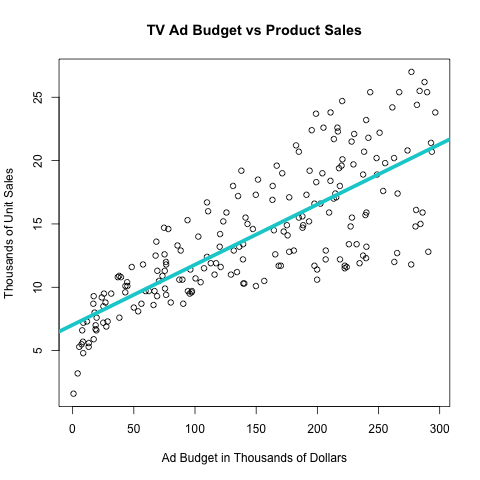
\includegraphics[width=160px]{../images/scatterplot-tv-sales.png}
\label{fig:scatterplot}
\end{figure}

This shows that in practice, markets with small ad budgets do not have sales as high as the intercept of the linear model would suggest.  In general, this is a shortcoming of linear models:  any curvature to the data at all and the relationship becomes less reliable.  One can gleam some idea of how good a linear fit is at representing a relationship in data by calculating the following statistics about the fit.

\begin{table}[ht]
\centering
\begin{tabular}{|c|c|}
Statistic & Value \\ \hline
RSS & 3.259 \\
$R^2$ & 0.612 \\
$F$-stat & 312.145 \\
\end{tabular}
\caption{Goodness of Fit Statistics}
\end{table}

Residual sum of squares, or \emph{RSS}, is a statistic computed using the forumula $RSS = \sum_{i=1}^n (y_i - f(x_i))^2$, where the $y_i$ values are the true value of the sales for a given markey while the $f(x_i)$ values are the expected sales based on the TV ad budget according to our model.  The least-squares fit is the fit that finds $\beta_0$ and $\beta_1$ so as to make the RSS as small as possible. 

The $R^2$ statistic is a measure of how closely the data falls along the regression line.  If all data points were perfectly along this line, $R^2 = 1$.  Instead, we have $R^2 = 0.612$.

The F-statistic displayed above is the ratio 

\begin{equation}
F = \frac{\mbox{Mean Squared Error of }f(x_i) \mbox{values}}
               {\mbox{Mean Squared Error of Error terms }{(y_i - f(x_i))}}
\end{equation}
and could be used if desired to asses goodness of fit using an F-test.

\section{Conclusions}

Clearly, the linear regression model fits this data well, but certainly not perfectly. An $R^2$ value of $0.612$ means the line fits the data reasonably well as $0.612 > 0.5$.  This means that for the majority of markets, increasing the TV ad budget for a product by \$1000 will result in an increase in sales of about $0.048$ units. 


\end{document}
